\chapter{Methods}

\section{DNA intercalator models}

% talk about the crystal structure and the experimental values in the other paper.
All systems that were simulated in this thesis started out from an x-ray crystal structure model. The nucleic acid database \cite{berman1992nucleic} contains 402 structures that are tagged as drug-DNA complexes. Just a few of these are high quality intercalated structures. After careful manual filtering and investigation we selected a set of 10 crystal structures to conduct docking and free energy calculation studies with.

The experimental data for the binding affinity of a molecules was from an experimental study done by Shibinskaya et al.\cite{shibinskaya2011synthesis}. The intercalators probed experimentally there were a congeneric series of molecules based on a common quinoxaline scaffold. To prepare this system in silico, we compared the molecule with the intercalators found in the crystal structures from the nucleic acid database. The crystal structure with ID 1Z3F had an intercalator with a very similar scaffold to quinoxaline, therefore is was chosen as the base of our model.

First the original intercalator was removed from the model, leaving just the DNA double stranded helix with an opening between two of the consecutive basepairs where the molecule was intercalating. Then we docked in the new intercalators with the OpenEye OEDocking toolkit \cite{kelley2015posit}. The docking method that we used was extensively validated, and we believed that the resulting model was a good starting point for the free energy calculations.    

\begin{figure}
  \centering
  \subfloat[1Z3F] {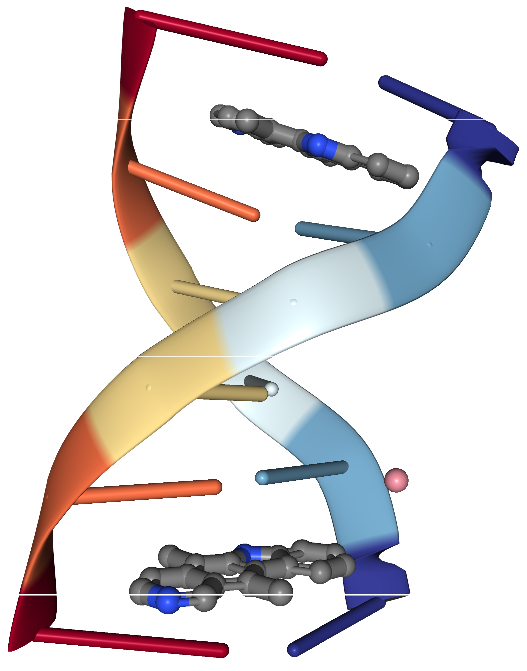
\includegraphics[scale=0.2]{1z3f}}%
  \subfloat[1G3X] {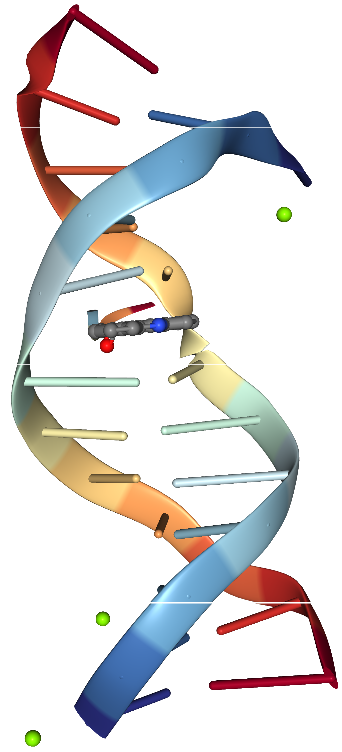
\includegraphics[scale=0.2]{1g3x}}%
	\subfloat[1HX4] {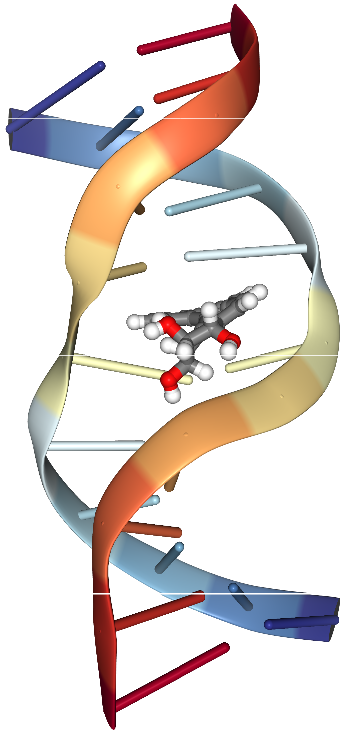
\includegraphics[scale=0.2]{1hx4}}
	
	\subfloat[2ROU] {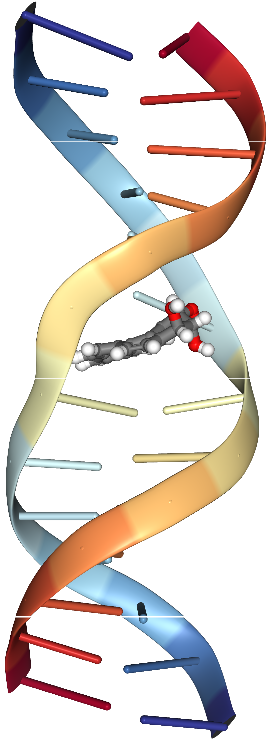
\includegraphics[scale=0.2]{2rou}}%
	\subfloat[1D11] {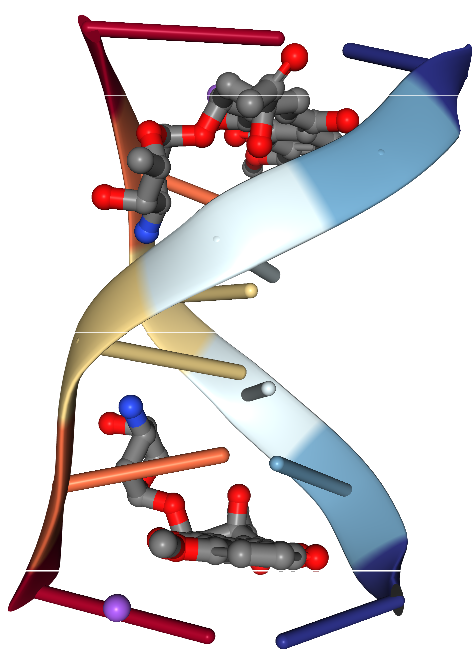
\includegraphics[scale=0.2]{1d11}}%
	\subfloat[1D12] {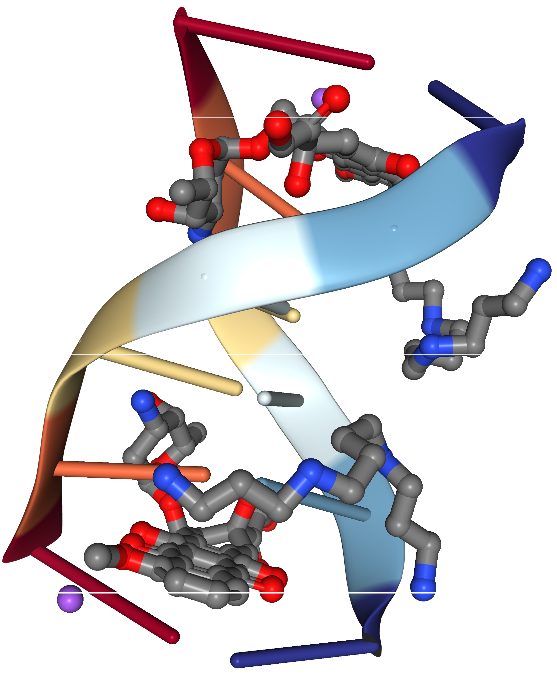
\includegraphics[scale=0.2]{1d12}}%
	
  \caption{Examples of the crystal structures found in the nucleic acid database. They all contain intercalators (one or two) somewhere in-between two basepairs. Structure with ID 1Z3F was used to as the starting point for modelling the experimentally found system in the simulations.}
  \label{}
\end{figure}

\begin{figure}
	\centering
	\subfloat[4 ring scaffold] {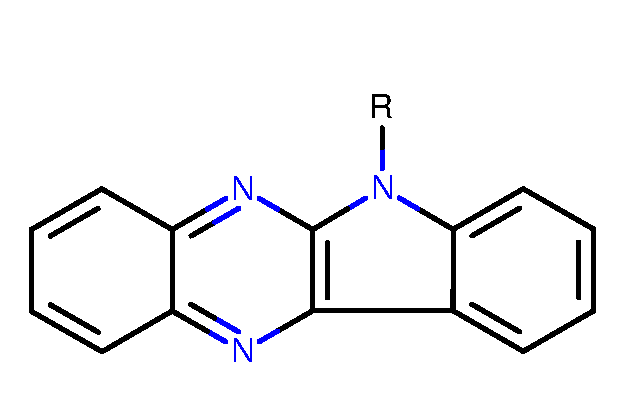
\includegraphics[scale=0.4]{interc1.pdf}}%
	\subfloat[5 ring scaffold] {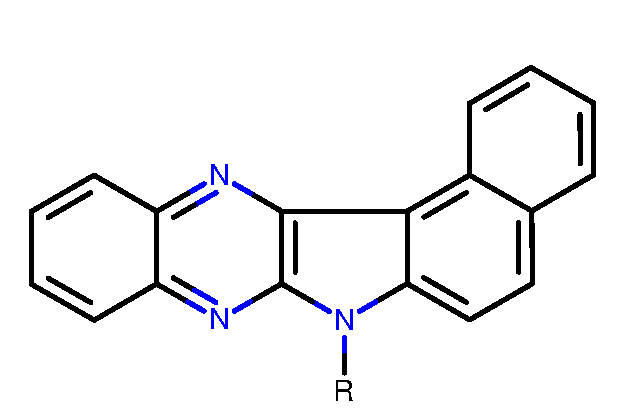
\includegraphics[scale=0.4]{interc2.pdf}}
	
	\subfloat[Side chains] {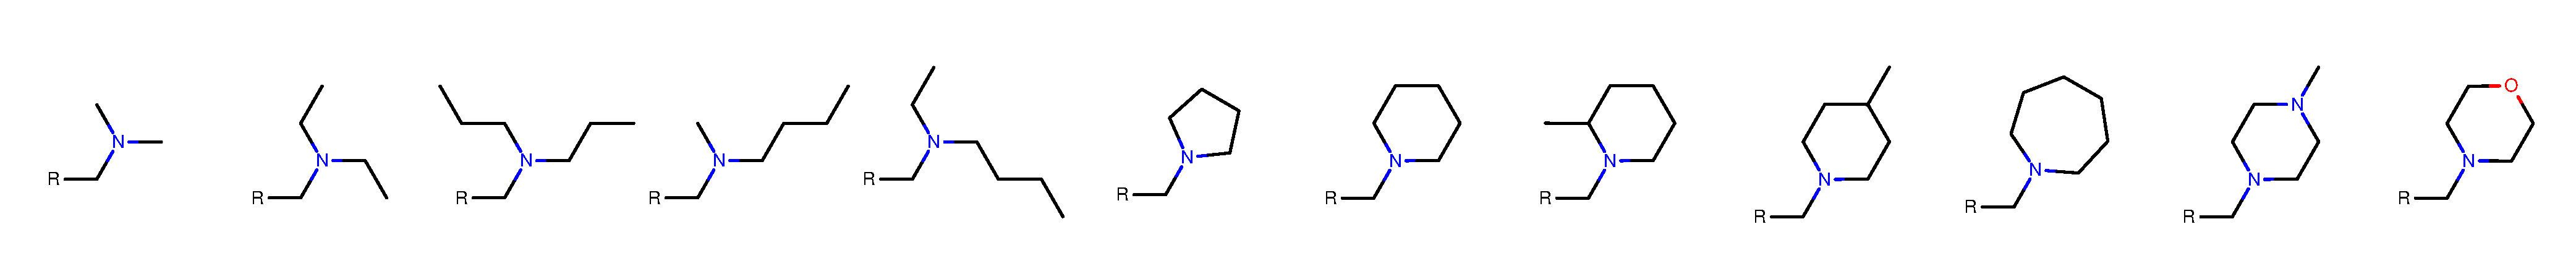
\includegraphics[width=\textwidth]{intercalators.pdf}}
	
	\caption{A congeneric series of DNA intercalators. All molecules share a common quinoxaline scaffold with both the 4 and 5 ring scaffold probed experimentally.}
	\label{fig:intercalators}
\end{figure}

The intercalators were generated from SMILES strings using OpenEye toolkit \cite{hawkins2010conformer}. First up to 1000 different conformations were generated with OEOmega with a maximum root mean square deviation of 2 angstrom. Then AM1BCC charges were assigned to them electronically least interacting functional groups method to select preferred conformers.

\section{Docking and scoring}

For certain application, like that of high throughput screening in the pharmaceutical industry, it is important to assess the binding strenght of a large number of drugs or molecules bound to large biological macromolecules like proteins or DNA in a very fast manner. This is done via easily evalutable scoring function, some notable examples including: AutoDock \cite{trott2010autodock}, X-Score \cite{wang2002further}, ChemScore \cite{eldridge1997empirical}, and others. Generally speaking, they take into account a single structure and little or no protein movement is taking into account during evaluation. One of the simplest scoring function  consists of the empirical surface-area based method that shows that ligand binding reduces the surface are in the receptor that is accessible to the surrounding solvent. The function makes the assumption that the polar and non-polar area on the surface of the molecule has a linear relation to the free energy. Due to the crude simplifications in these models, they have weak predictive power and are rarely used for accurate free energy estimation. Here, a scoring methods is used for two reasons: (i) to find an initial structure for the intercalator-DNA complex, and (ii) to compare the scores and hence the ranking of this methods with other, more accurate models. Docking and scoring has its place in the drug discovery pipeline. In high throughput scenarios, where speed is an important factor due to the large number of molecules that need to be tested, scoring functions are often used to filter out candidates that have low probability of being good binders \cite{mobley2009binding}.

In this thesis we used the ChemScore scoring function as implemented in OpenEye OEDocking toolkit. We always ran an exhaustive docking search with all the generated conformations of the intercalators as possible good fits. Docking was restricted to a large box around the two consecutive base pairs with additional padding to fit in any molecule side chains if present. 


\section{ESMACS}

The molecular dynamics package OpenMM \cite{eastman2017openmm} was used throughout the minimisation, equilibration and production phases of the simulations. The minimisation phase was conduced using the conjugate gradient algorithm in OpenMM for 1000 iterations.

Non-bonded interactions were cut off at 12 angstrom and long range Coulomb interactions were handled using the Particle Mesh Ewald (PME) method. In order to obtain an integration timestep of 2 fs the settle \cite{miyamoto1992settle} algorithm was applied to all atoms covalently bonded to hydrogen atoms in both the equilibration and production simulations.

During equilibration the system was maintained at 300 K and 1 atm using the Langevin thermostat and Monte Carlo Barostat implemented in OpenMM with default settings. This resulted in the system sampling an isothermal isobaric (NPT) ensemble. Equilibration was done for 4 ns.

The equilibrated systems were kept in the same isothermal isobaric ensemble as the final state of the equilibration. All ensemble simulation were run for 16 ns simulation time. In total we ran each protocol for 25 replicas.


\section{TIES}

The complexes of target DNA and hybrid intercalators were solvated in an orthorhombic water box with buffer width of 11 angstrom. The system was neutralized electrostatically with counterions. The BSC1\cite{ivani2016parmbsc1} force field was employed in all our simulations for DNA parameters. Intercalator parameters were produced using the general AMBER force field 2 (GAFF2) \cite{wang2004development}. The AM1BCC \cite{jakalian2002fast} %
semi-empirical methods was used to produce the partial charges on the intercalator atoms (AmberTools 18 \cite{ambertools18}) after geometry optimization with the OpenEye OEGauss toolkit. The simulation engine NAMD 2.12 was used for producing all the trajectories of the complex systems with periodic boundary conditions. The system was brought to and maintained at a temperature of 300 K and 1 atmosphere using the NAMD implementation of the Langevin thermostat (with a damping coefficient of $5 ps^{-1}$) and a Berendsen barostat (compressibility of $4.57 \times 10^{-5} bar^{-1}$ and a relaxation time of $100 fs$). The time step was set to $2 fs$. The van der walls terms perturbed linearly with respect to $\lambda$. To avoid end point catastrophes were atoms near the end point appear suddenly too close to each other a soft core potential was used for the van der Walls interactions. The electrostatic interactions of the disappearing atoms are linearly decoupled until $\lambda = 0.55$ then completely turned off afterwards, and those atoms that are appearing are electrostatically turned on from $\lambda = 0.45$ linearly increasing until the end.

All calculations were done with 13 $\lambda$ windows. At each value of $\lambda$ 5 replica simulations were run to assess the error. For each replica, the standard protocol for minimisation and equilibration was performed, that is 4 ns of simulation time. Production runs for each replica were 16 ns long. While the coordinates were recorded every 10 ps, $\partial V / \partial \lambda$ values were recorded every 2 ps. The choice of 16 ns for the simulation length and 5 for the ensemble size is based on the uncertainty quantification and error analysis discussed in the previous work. The protocol described here can be adjusted to the specific system at hand, but this was enough to converge results for all of the systems in this study. The size of the ensemble can be adjusted even at specific windows to account for additionally uncertainty that may arise. The TIES workflow can be executed in an embarrassingly parallel fashion, and given sufficient resources the simulations can finish in 15 hours. In general the turnaround time depends on the system size, number of cores used per simulation instance with GPUs offering additional speedup.

\section{Large scale adaptive binding free energy calculations}

To enable the running of large amounts of simulations on supercomputers we developed the high throughput binding affinity calculator (HTBAC). The architecture of HTBAC and its uses is described here, and published in more detail in the proceedings of the 2018 eScience IEEE conference.
 
HTBAC is a software system for running ensemble-based free energy protocols adaptively and at scale on HPC resources. Currently, HTBAC supports protocols composed of an arbitrary number of analysis and simulation steps, and relies on the ensemble management system and runtime system provided by the RADICAL-Cybertools (RCT). HTBAC is designed to be extended to support more types of protocols and alternative runtime middleware.

\subsection{Design and implementation}

HTBAC exposes four constructs to specify free energy protocols: Protocol, Simulation, Analysis, and Resource. Protocol enables multiple descriptions of protocol types, while Simulation and Analysis specify simulation and analysis parameters for each protocol. Resource allows to specify the amount of resources needed to execute the given protocols. Together, protocol instances, simulation and analysis parameters, and resource requirements constitute an HTBAC application.
In HTBAC, each protocol models a unique protein ligand physical system. Each protocol follows a sequence of simulation and analysis steps, assigning ensemble members to execute independent simulations or analysis. An ensemble member that executes an independent simulation within a simulation step is referred to as a replica. Each simulation is assigned a different initial velocity, which enables simulations to begin in different parts of the ligand’s phase space.
Individual simulations or analyses with input, output, termination criteria and dedicated resources are designed as a computational task. Aggregates of tasks with dependencies that determine the order of their execution constitute a workflow. In this way, HTBAC encodes NP instances of the Pth protocol as a workflow of computational tasks.
Fig. ~\ref{fig:htbac} shows the components and subcomponents of HTBAC. HTBAC API enables users to codify protocol descriptions in terms of protocol type, simulation and analysis steps, and computer infrastructure requirements. Descriptor uses two subcomponents to aggregate protocol descriptions into a single application and resource description. Note that Descriptor can aggregate different types of protocols, with different computing and resource requirements.
Runner has three subcomponents: Execution Manager, Middleware Connector and Runtime Adaptive Evaluator. Execution Manager communicates with the execution layer via a connector to coordinate the execution of the application. In principle, HTBAC can use multiple connectors for diverse middleware to access different computing infrastructures.
Middleware Connector converts the application description of HTBAC into a middleware-specific format. Execution Manager can pass the given application to the connector in full or only in parts. This enables to start the execution of an application before its full description is available or to
change those parts of the application that still have to be executed. This will enable future capabilities like, for example, to concurrently execute the application on diverse middleware.
Runtime Adaptive Evaluator enables the execution of adaptive applications. This subcomponent can evaluate partial results of an application execution via tailored algorithms. On the base of this evaluation, Runtime Adaptive Evaluator can decide to return the control to Execution Manager or to modify the description of the application that is being executed. In this way, HTBAC implements adaptivity for diverse protocols, allowing users to define arbitrary conditions and algorithms.
HTBAC is implemented in Python as a domain-specific library. All components of HTBAC are implemented as objects that communicate via method calls. HTBAC uses two RCT as building blocks: Ensemble Toolkit (EnTK) and RADICAL-Pilot (RP).
EnTK provides HTBAC capabilities to execute ensemble-based applications. EnTK exposes three constructs: Task, Stage and Pipeline. Tasks contain information regarding an executable, its software environment and its data dependencies. Stages are sets of tasks without mutual dependencies that can execute concurrently. Pipeline are lists of stages, where stages can execute only sequentially and each pipeline can execute independently. HTBAC uses a Middleware Connector for EnTK to encode a protocol instance as a single pipeline that contains stages of individual simulations and analyses tasks.
EnTK uses RP to execute tasks via pilots. RP supports task level parallelism and high-throughput by acquiring resources from a computing infrastructure and scheduling tasks on those resources for execution. Pilot systems execute tasks directly on the resources, without queuing them on the infrastructure’s scheduler.

\subsection{Adaptivity}

The design of HTBAC permits enhancing protocols while continuing to use ``static'' simulation engines. To this end, we implemented two adaptive methods using HTBAC: adaptive quadrature and adaptive termination. Both of these methods use the features of adaptivity offered in HTBAC to scale to large number of concurrent simulations and to increase convergence rate and obtain more accurate scientific results.
The aim of introducing adaptive quadrature for alchemical free energy calculation protocols (e.g., TIES) is to reduce time to completion while maintaining (or increasing) the accuracy of the results. Time to completion is measured by the number of core hours consumed by the simulations. Accuracy is defined as the error with respect to a reference value, calculated via a dense $\lambda$ window spacing (65 windows). This reference value is used to establish the accuracy of the non-adaptive protocol (which has 13 $\lambda$ windows) and the adaptive protocol (which has a variable number of $\lambda$ windows, determined at run time).
One of the input parameters of the adaptive quadrature algorithm is the desired acceptable error threshold of the estimated integral. We set this threshold to the error of the non-adaptive algorithm calculated via the reference value. The algorithm then tries to minimise the number of $\lambda$ windows constrained by the accuracy requirement.
